\subsection{旋转构建杯零件三维模型}
现在,我们用\ref{sec:beilingjiantezheng}节绘制的图形来构建杯零件的三维模型。
\begin{procedure}
\item 对图\ref{fig:bettezheng}所示的图形进行面域操作,若采用集合法绘制图\ref{fig:bettezheng}所示的图形,则不可跳过此步骤。
启动面域命令后,要求选择用于构建面域的图线。此时,用鼠标拾取图形中一条图线,被选中的线段会以虚线形式表示,结果如图\ref{fig:regionselecta}所示。
\begin{lstlisting}
|命令:REGION|
|选择对象: 找到 1 个|
\end{lstlisting}
继续拾取图形中剩下图线,构成图\ref{fig:regionselectb}所示的虚线表示的封闭框。
\begin{lstlisting}
|选择对象: 找到 1 个,总计 2 个|
|选择对象: 找到 1 个,总计 3 个|
|选择对象: 找到 1 个,总计 4 个|
|选择对象: 找到 1 个,总计 5 个|
|选择对象: 找到 1 个,总计 6 个|
|选择对象:|
\end{lstlisting}
面域成功后,整个图形构成了一个整体。若用鼠标拾取该图形,只需要点选一次就以选择中整个图形。
\begin{figure}[htbp]
\centering
\subfloat[]{\label{fig:regionselecta}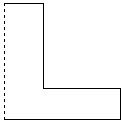
\includegraphics[scale=1.2]{regionselect1.png}}\hspace{30pt}
\subfloat[]{\label{fig:regionselectb}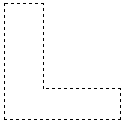
\includegraphics[scale=1.2]{regionselect.png}}
\caption{面域对象选择}
\end{figure}
\item 构建杯零件三维模型。用旋转建模法构建实体需要用到实体旋转命令。实体【旋转】命令的启动方法有:
\begin{itemize}
\item 键盘输入revolve\index{revolve}或rev。
\item 【绘图】$\rightarrow$【旋转】。
\item 【建模】$\triangleright$【旋转】图标
\includegraphics[scale=0.6]{solidrevolve.png}。
\end{itemize}
启动命令后,要求选择用于旋转操作的对象。此时,用鼠标选取面域好的对象,并结束选择。
\begin{lstlisting}
|命令: REVOLVE|
|当前线框密度:  ISOLINES=4,闭合轮廓创建模式 = 实体|
|选择要旋转的对象或 [模式(MO)]: 找到 1 个|
|选择要旋转的对象或 [模式(MO)]:|
\end{lstlisting}
接下来需要定义用于旋转的中心线。用捕捉方式选择图\ref{fig:revnodeselecta}所示的端点为中心线的第一个点,图\ref{fig:revnodeselectb}所示的端点为中心线的第二个点,构成旋转中心轴线。
\begin{lstlisting}
|指定轴起点或根据以下选项之一定义轴 [对象(O)/X/Y/Z]$<$对象$>$:|
|指定轴端点:|
\end{lstlisting}
最后指定旋转角度,其默认值是360度。
\begin{lstlisting}
|指定旋转角度或 [起点角度(ST)/反转(R)/表达式(EX)] $<360>$:|
\end{lstlisting}

\begin{figure}[htbp]
\centering
\subfloat[选择第一个端点]{\label{fig:revnodeselecta}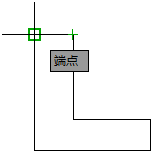
\includegraphics[scale=1]{revnodeselect1.png}}\hspace{30pt}
\subfloat[选择第一个端点]{\label{fig:revnodeselectb}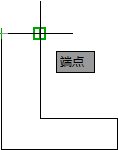
\includegraphics[scale=1]{revnodeselect2.png}}
\caption{旋转中心定义}
\end{figure}
\item 将视图切换为【西南等轴测】,并将【视觉样式】设置为【灰度】即可得到图\ref{fig:beimodel}所示的调压阀杯零件三维模型效果。
\begin{figure}
\centering
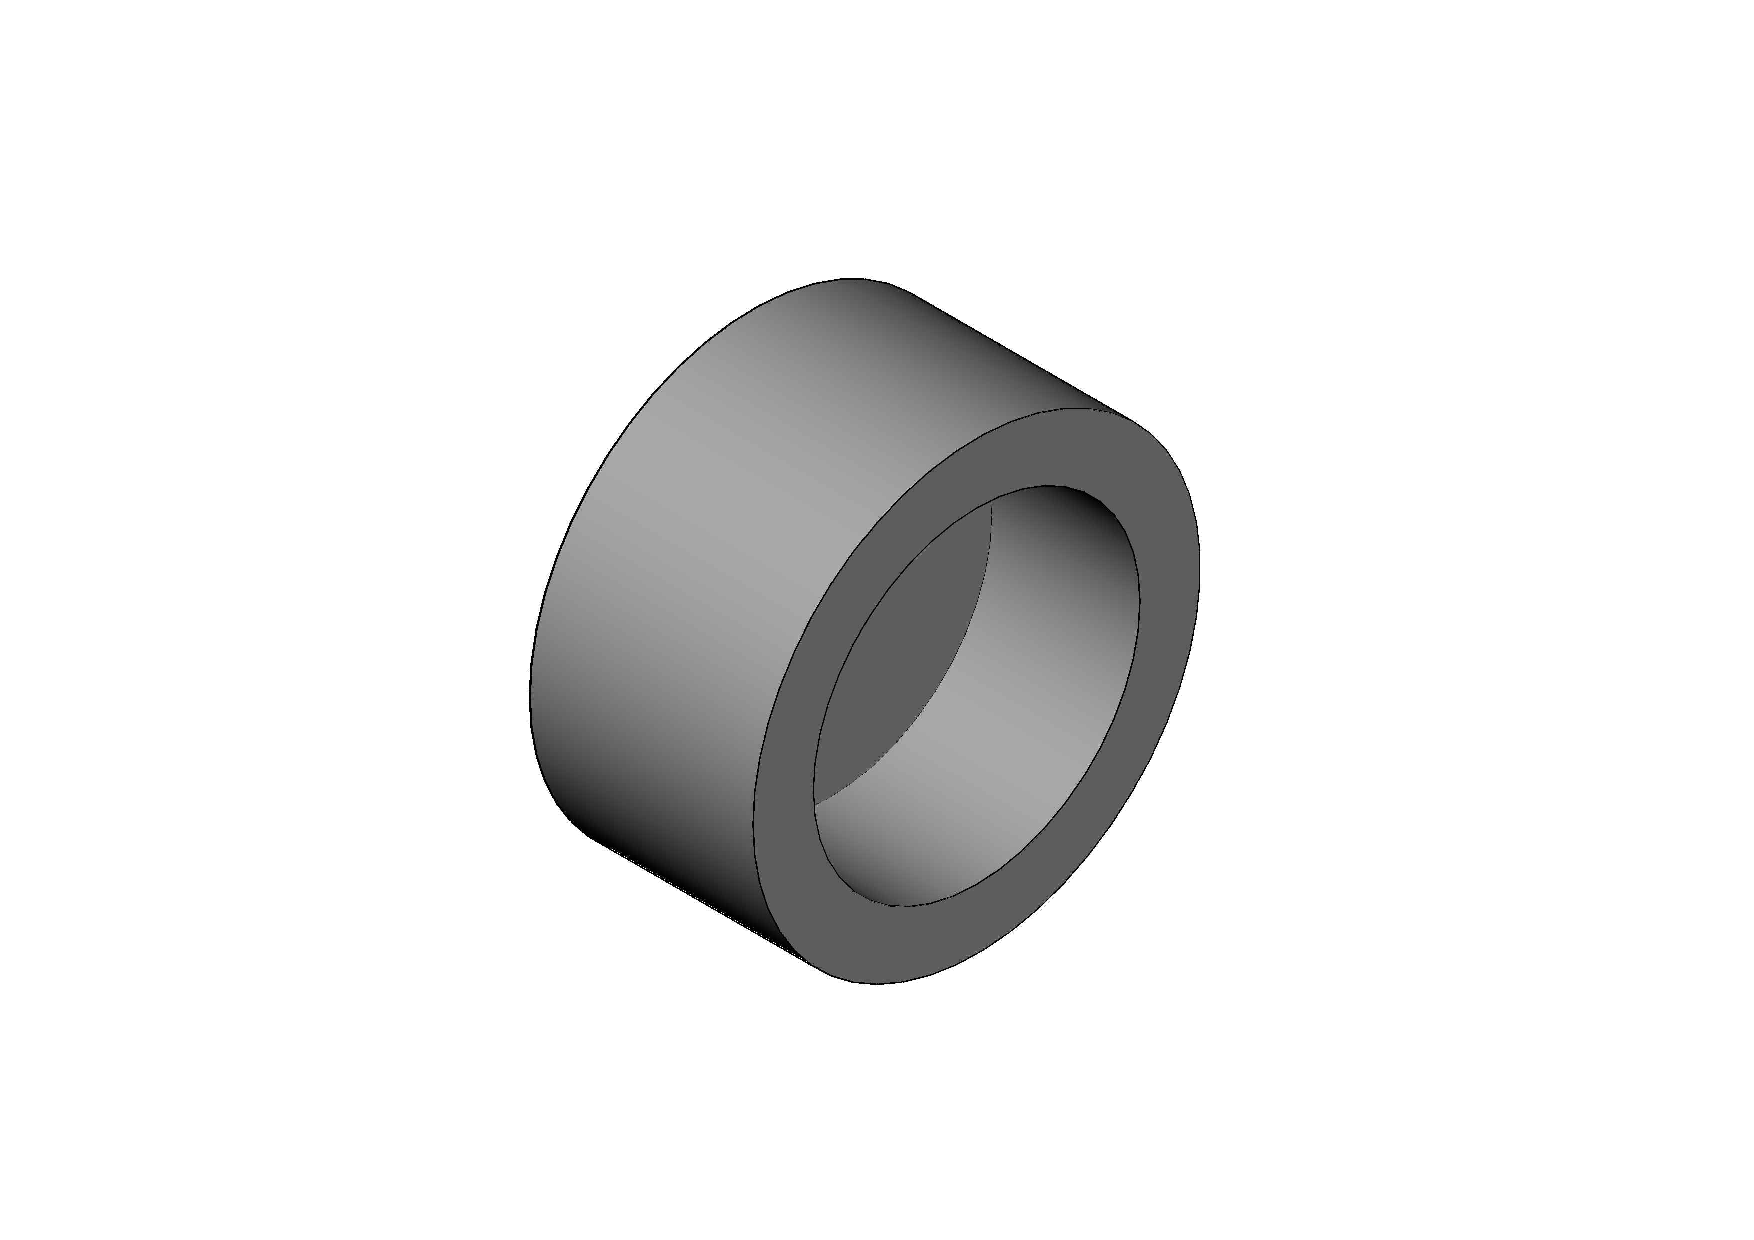
\includegraphics[scale=0.6]{beimodel.pdf}
\caption{杯零件三维模型}\label{fig:beimodel}
\end{figure}
切换【西南等轴测】的方法有:
\begin{itemize}
\item 键盘输入-VIEW或-V,并输入SWISO。
\item 【视图】$\rightarrow$【三维视图】$\rightarrow$【东南等轴测】。
\item 【视图】$\triangleright$【西南等轴测】图标
\includegraphics[scale=0.6]{estool.png}。
\end{itemize}
设置【视觉样式】的方法是:
\begin{itemize}
\item  键盘输入VSCURRENT\index{vscurrent},选择【灰度G】项。
\item 【视图】$\rightarrow$【视觉样式】$\rightarrow$【灰度】。
\end{itemize}
\item 将文件保存为“杯块零件三维图.dwg”。AutoCAD保存文件的方法有:
\begin{itemize}
\item 键盘输入SAVE\index{save}或SAVEAS\index{saveas}。
\item 键盘输入\fbox{Ctrl}+\fbox{S}。
\item 【文件】$\rightarrow$【保存】或【另存为】。
\item 【工具栏】$\triangleright$【保存】图标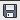
\includegraphics[scale=0.6]{savetool.png}。
\end{itemize}
\end{procedure}
\begin{figure}[htbp]
\centering
\subfloat[]{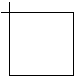
\includegraphics[scale=1.6]{regerror1.png}}\hspace{20pt}
\subfloat[]{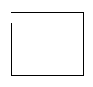
\includegraphics[scale=1.6]{regerror2.png}}\\
\subfloat[]{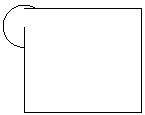
\includegraphics[scale=1]{regerror3.png}}\hspace{20pt}
\subfloat[]{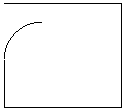
\includegraphics[scale=1]{regerror4.png}}
\caption{不能成功创建面域的情况}\label{fig:buchengong}
\end{figure}

面域操作和实体旋转操作需要注意地方和技巧。
\begin{tips}
\item 【面域】命令要求选择的线段必须构成封闭线框,即要求如图\ref{fig:regionselectb}一样,所选择的线段要首尾相接,否则将不能成功创建面域。
\item 图\ref{fig:buchengong}所示的几种情况都不能够成功创建面域。

\item 实体【旋转】命令的角度决定用选定的对象旋转多少度,例如90度将产生四分之一形状的回转体。默认情况下则为360度。
\item 使用实体【旋转】命令时,定义用于旋转的轴线必须位于
\end{tips}
\endinput